\section{Guia do Desenvolvedor}\label{RS0003:developer}

Neste guia serão apresentados procedimentos essenciais para o desenvolvedor que desejar customizar o Portal Institucional do ITA.

Para tal é necessário conhecimentos de:

\begin{itemize}
    \item \textbf{JavaScript} - \href{https://developer.mozilla.org/en-US/docs/Web/javascript}{https://developer.mozilla.org/en-US/docs/Web/javascript}
    \item \textbf{NodeJS} - \href{https://nodejs.org/en/}{https://nodejs.org/en/}
    \item \textbf{HTML} - \href{https://www.w3.org/html/}{https://www.w3.org/html/}
    \item \textbf{CSS} - \href{https://www.w3.org/Style/CSS/Overview.en.html}{https://www.w3.org/Style/CSS/Overview.en.html}
    \item \textbf{MongoDB} - \href{https://www.w3.org/Style/CSS/Overview.en.html}{https://www.w3.org/Style/CSS/Overview.en.html}
\end{itemize}

Além destes elementos essenciais, bibliotecas JavaScript são utilizadas para facilitar o uso destas tecnologias, e entre estas destacamos as seguintes ferramentas que também devem ser dominadas pelo desenvolvedor:

\begin{itemize}
    \item \textbf{ExpressJS} - Interface de programação entre a plataforma NodeJS e cliente no \gls{browser} - \href{http://expressjs.com}{http://expressjs.com}
    \item \textbf{HandlebarsJS} - Templates de páginas HTML - \href{https://handlebarsjs.com}{https://handlebarsjs.com}
    \item \textbf{Mongoose} - Interface de programação entre o banco de dados de documentos Mongo e aplicações NodeJS - \href{https://mongoosejs.com}{https://mongoosejs.com}
    \item \textbf{Winston} - Registro de eventos (``\textit{Logs}'') - \href{https://github.com/winstonjs/winston}{https://github.com/winstonjs/winston}
\end{itemize}

\begin{displayquote}\footnotesize
    De modo algum este guia pretende servir de instrução ou sequer introdução a qualquer uma das tecnologias listadas e toda e qualquer informação necessária para uso e configuração das mesmas deve ser obtido diretamente nas fontes apontadas acima ou em fontes adicionais que podem ser encontradas na internet
\end{displayquote}\normalsize

\begin{displayquote}\footnotesize
    \textbf{Atenção}: Listagens de trechos de código, ``\textit{scripts}'' e páginas HTML apresentados neste manual podem não corresponder à versão final do portal.

    Algumas das providencias tomadas para documentar o portal, foram por exemplo, reformatar o código para melhor apresentação neste manual, portanto diferenças básicas são esperadas.

    De qualquer modo, a versão utilizada para confecção deste manual é uma versão totalmente funcional, livre de falhas significativas e de acordo com os desejos dos tomadores de decisão que nos orientaram durante a construção do portal, 
    
    Qualquer diferença notada pode e deve ser considerada irrelevante a partir deste momento.
\end{displayquote}\normalsize

\subsection{Localizando-se}

\subsubsection{Estrutura de diretórios}

\begin{forest}
    pic dir tree,
    where level=0{}{
        directory,
    },
    [portal
        [assets
            [static
                [core
                    [css]
                    [js
                        [library]
                    ]
                ]
            ]
        ]
        [config]
        [helpers]
        [models]
        [routes
            [methods]
            [views
                [iex]
                [search]
            ]
        ]
        [translations]
        [views
            [iex]
            [layouts]
            [partials]
            [search]
        ]
    ]
\end{forest}

Estas pastas contém programas do portal e artefatos da camada de apresentação do portal.

\begin{itemize}
    \item ``\textit{assets / static }'' - o conteúdo ``estático'' do portal, ou seja, que não é formatado por código do portal
    \item ``\textit{config}'' - arquivos de configuração
    \item ``\textit{helpers}'' - rotinas de suporte comuns à diversas funções do portal
    \item ``\textit{models}'' - definições da estrutura de dados do portal (o conteúdo dinâmico produzido pelo portal)
    \item ``\textit{routes}'' - código do portal que processa as rotas de requisições (\gls{URL}) do navegador
    \item ``\textit{translations}'' - tradução dos termos comuns do portal (a tradução de páginas é feita à parte por meio da estrutura de dados)
    \item ``\textit{views}'' - definições da camada de apresentação (contém a forma e direciona o conteúdo apresentado pelo portal)
\end{itemize}

Estas são as principais pastas com que o desenvolvedor deve se ocupar para customizar o Portal Institucional. Maiores detalhes serão apresentados nas seções à seguir. 

Além destas, outras pastas de trabalho são criadas para conteúdo e bibliotecas do Portal.

\begin{forest}
    pic dir tree,
    where level=0{}{
        directory,
    },
    [portal
        [assets
            [static
                [core
                    [uploads
                        [Archive]
                        [Menu]
                        [Post]
                        [Spotlight]
                    ]
                ]
            ]
        ]
        [log]
        [node\_modules]
    ]
\end{forest}

\begin{itemize}
    \item ``\textit{assets / core / uploads}'' - contém arquivos que foram inseridos no conteúdo do portal por editores
    \item ``\textit{log}'' - arquivos com registros de ocorrências do portal
\end{itemize}

Estes arquivos podem ser configurados e residir em outra estrutura de arquivos do servidor.

\subsection{Configuração}

O Portal Institucional possui diversos arquivos de configuração e parte da customização é feita por meio de ajustes nestes arquivos.

\begin{forest}
    pic dir tree,
    where level=0{}{
        directory,
    },
    [portal
        [config
            [cookies.js, file]
            [default.js, file]
            [editor.js, file]
            [headers.js, file]
            [rules.js, file]
        ]
    ]
\end{forest}

Além destes arquivos, o ``\textit{Script}'' de inicialização do sistema operacional carrega definições particulares do ambiente de execução (ver Guia do Operador).

\begin{itemize}
    \item $cookies.js$ - habilita a opção de apresentar uma mensagem solicitando permissão de uso de ``\textit{Cookies}'' pelo Portal
    \item $default.js$ - configurações comuns e gerais
    \item $editor.js$ - configuração do editor de texto utilizado para criar e atualizar publicações
    \item $headers.js$ - configuração dos cabeçalhos \gls{HTML}
    \item $rules.js$ - configurações de regras de acesso
\end{itemize}

\subsection{Customizando o Portal}

O Portal Institucional é amplamente customizável por um desenvolvedor com conhecimentos de HTML e CSS e algum conhecimento básico de JavaScript.

Um desenvolvedor com conhecimento mais profundo de JavaScript e a plataforma NodeJS poderá transformar totalmente o portal.

Antes de mais nada, para construção do portal, foram utilizados algumas ferramentas básicas, todas elas incorporadas e customizadas, ou seja, o Portal Institucional é o resultado de ampla e profunda customização de outros projetos de código livre na internet.

A principal ferramenta utilizada é o \gls{CMS} \href{https://www.keystonejs.com}{Keystone}. Nossa customização chama-se ``\textbf{CapstoneJS}'' e foi baseada na versão 4 do projeto ``\textbf{KeystoneJS}'' original. Tanto que a documentação original daquele projeto pode ser utilizada como referência para a nossa versão (veja em \href{https://v4.keystonejs.com/documentation/}{https://v4.keystonejs.com/documentation/})\footnote{A principal razão para termos realizado o que se chama ``\textit{fork}'' deste projeto é que a versão 4 foi descontinuada e a versão 5 é completamente incompatível, e como necessitamos implementar melhorias e correções que os desenvolvedores originais não mais estão disponíveis para fazê-las}.

Esta implementação, apesar de permitir a gestão de conteúdo dinâmico para um Portal, não pode ser classificada como um \gls{CMS} completamente funcional pois isto vai muito além do escopo de um Portal de conteúdo para uma instituição de ensino superior, faltando neste alguns dos recursos encontrados em produtos do mercado tais como:

\begin{itemize}
    \item Taxonomia, ou a criação hierárquica de classes de informações e a classificação de publicações dentro destas classes e a hierarquização de conteúdo
    \item Indexação completa e compreensiva por autores, data, taxonomia, etc.
    \item Gerenciamento de formatos de apresentação
    \item Controles de revisão de documentos
    \item Gerenciamento de sistema de arquivos, armazenamento de documentos, conversão de formatos de documentos, importação de documentos
    \item Gerenciamento de ``\textit{templates}'' de apresentação de conteúdo, customização de ``\textit{templates}''
    \item Inclusão de comentários de leitores e de grupos de discussão
    \item Controle de versionamento
    \item Gerenciamento muli-idiomas customizável
\end{itemize}

Porém este Portal implementa de modo limitado algumas destas funcionalidades:

\begin{itemize}
    \item Inclusão de conteúdo dinâmico a ser publicado pelo Portal com um editor \gls{HTML} \gls{WYSIWYG} simples
    \item Tradução de conteúdo por meio de seleção do idioma desejado no Painel (limitada aos idiomas disponibilizados via configuração - ver Guias de Operação e Desenvolvimento)
    \item Configuração de regras de acesso e perfis de usuário
    \item Importação de arquivos para serem baixados pelos leitores
    \item Importação de imagens para serem apresentadas no conteúdo estático
\end{itemize}

Além do ``\textbf{CapstoneJS}'' implementamos também:

\begin{itemize}
    \item ``\textit{capstone-accesscontrol}'' - baseado no projeto \href{https://github.com/onury/accesscontrol}{``\textit{onury / accesscontrol}''} faz controle de acesso para edição de conteúdo do portal integrado ao ``\textit{CapstoneJS}''
    \item ``\textit{capstone-file-manager}'' - faz a mesma função do componente \href{https://github.com/Sidenis/keystone-file-manager#readme}{``\textit{Sidenis / KeystoneJS file manager}''} que permite aos editores inserir arquivos para serem baixados pelos usuários que navegam no portal
    \item ``\textit{capstone-intl}'' - versão customizada para o ``\textit{CapstoneJS}'' do componente \href{https://github.com/alexsk/mongoose-intl}{``\textit{alexsk / mongoose-intl}''} que permite inserir conteúdo multi-idioma em estruturas de dados do MongoDB
\end{itemize}

São principalmente estas mudanças e implementações adicionais que explicaremos aqui, e para maiores informações sobre como usar estes componentes, basta acessar os projetos originais e buscar na documentação.

\subsubsection{A construção de uma rota}

Rotas são \glspl{URI} que apresentam o conteúdo do portal de modo específico.

\begin{forest}
    pic dir tree,
    where level=0{}{
        directory,
    },
    [portal
        [config]
        [routes
            [methods
                [download.js, file]
                [search.js, file]
            ]
            [views
                [iex
                    [local.js, file]
                    [region.js, file]
                ]
                [search
                    [gallery.js, file]
                    [posts.js, file]
                ]
                [about.js, file]
                [home.js, file]
                [post.js, file]
            ]
            [index.js, file]
        ]
    ]
\end{forest}

As rotas são ``configuradas'' no arquivo $config / default.js$ conforme podemos ver na linha $85$ da \cref{RS0003:code:conf-routes}.

\begin{code}
    \inputminted[label=default.js,firstline=83,lastline=86]{JavaScript}{../RS0003/anexos/default.js}
    \caption{Configuração das rotas}\label{RS0003:code:conf-routes}
\end{code}

As rotas são ``definidas'' no arquivo $routes / index.js$ (veja \cref{RS0003:code:def-routes}).

\begin{code}
    \inputminted[label=index.js,firstline=105,lastline=115]{JavaScript}{../RS0003/anexos/index.js}
    \caption{Definição das rotas}\label{RS0003:code:def-routes}
\end{code}

A definição da rota segue o método padrão adotado pelo \textbf{ExpressJS}, onde o padrão da requisição da \gls{URI} é informado, seguido do ``\textit{Middleware}'' padrão de proteção do \textbf{Capstone} (aka \textbf{Keysonte}), seguido do caminho para o programa em \textbf{JavaScript} com a implementação da rota.

Aas rotas fixas listadas na \cref{RS0003:code:def-routes} se referem à:

\begin{enumerate}
    \setcounter{enumi}{115}
    \item $search$ - pesquisa de publicações
    \item $gallegy$ - listagem de publicações com disposição em quadros com várias linhas e colunas
    \item $geral$ - a página de apresentação da instituição
    \item $iex$ - lista de regiões dos acordos internacionais da \textbf{IPR}
    \item $ies/local$ - lista local de acordos da \textbf{IPR}
    \item $post$ - mostra uma publicação
    \item $posts/category$ - lista todos as publicações de uma determinada categoria
\end{enumerate}

\begin{displayquote}
    Observe que a notação $routes.methods.search$ equivale ao caminho para a pasta $routes / methods / search$
\end{displayquote}

Por exemplo, a rota $/:lang?/geral$ aponta para $routes.views.about$. Nas listagens \ref{RS0003:code:about-1},  \ref{RS0003:code:about-2} e  \ref{RS0003:code:about-3} vemos a implementação completa.

\begin{code}
    \inputminted[label=about.js,firstline=1,lastline=18]{JavaScript}{../RS0003/anexos/about.js}
    \caption{Implementação de uma rota}\label{RS0003:code:about-1}
\end{code}

Em \ref{RS0003:code:about-1} fazemos a inicialização da rota. O componente $app-module-path$ facilita localizar todos os componentes que estão na pasta $helpers$. Em seguida instanciamos dois componentes essenciais para toda rota:

\begin{itemize}
    \item $partials$ - contém ``partes'' das páginas do portal que juntas formam a apresentação completa do conteúdo desejado
    \item $capstone$ - o gerenciador de conteúdo
\end{itemize}

Em seguida, na linha $7$ inicializamos o gerenciador de conteúdo (\textbf{CapstoneJS}) e da linha $9$ até $17$ as variáveis que irão conter o conteúdo apresentado.

\begin{code}
    \inputminted[label=about.js,firstline=18,lastline=60]{JavaScript}{../RS0003/anexos/about.js}
    \caption{Implementação de uma rota}\label{RS0003:code:about-2}
\end{code}

Prosseguimos resgatando o conteúdo do portal usando as rotinas em $partials$ da linha $19$ até $59$. O conteúdo resgatado é atribuído às variáveis definidas nas linhas $9$ até $17$.

\begin{code}
    \inputminted[label=about.js,firstline=60,lastline=62]{JavaScript}{../RS0003/anexos/about.js}
    \caption{Implementação de uma rota}\label{RS0003:code:about-3}
\end{code}

Finalmente, na linha $61$, solicitamos ao \textbf{CapstoneJS} para apresentar a página desejada.

Na seção a seguir iremos apresentar como resgatar conteúdo parcial e sem seguida como compor uma página.

\subsubsection{Resgate de um conteúdo parcial}

Vimos que durante o processamento de uma rota, informações dos dados a serem apresentados pelas páginas do portal como conteúdo dinâmico são resgatados em pequenas porções que chamamos de ``parciais''.

Estas ``parciais'' estão todas definidas no programa $helpers / partials.js$. Vamos ver a seguir como definir uma parcial.

\begin{code}
    \inputminted[label=partials.js,firstline=60,lastline=71]{JavaScript}{../RS0003/anexos/partials.js}
    \caption{Implementação de uma parcial}\label{RS0003:code:partial}
\end{code}

A \cref{RS0003:code:partial} lista o resgate de um ``\textit{Post}'' (postagem ou publicação), que é o elemento central de um gerenciador de conteúdo. Na linha $61$ a partial é definida recebendo os parâmetros $query$, $language$ e $callback$ (ela segue o padrão de rotinas assíncronas do \textbf{NodeJS}).

Em $query$ recebemos uma expressão que irá pesquisar no banco de dados \textbf{MongoDB} pelo ``\textit{Post}'' que desejamos. Apenas um único ``\textit{Post}'' será resgatado por esta rotina (outras parciais resgatam mais de um). Esta expressão obedece os critérios de expressões do \textbf{MongoDB} e \textbf{Mongoose}.

Em seguida o parâmetro $language$ é o código de linguagem para o qual o resultado deve ser traduzido pelo gerenciador de conteúdo. Finalmente, o parâmetro $callback$ contém uma função em \textbf{JavaScript} que irá receber a resposta da consulta quando esta estiver pronta (padrão de chamadas assíncronas do \textbf{NodeJS}).

Olhando nas linha $27$ da \cref{RS0003:code:about-2} podemos ver uma chamada à esta parcial (trecho que reproduzimos à seguir).

\begin{code}
    \inputminted[label=about.js,firstline=25,lastline=32]{JavaScript}{../RS0003/anexos/about.js}
    \caption{Implementação de uma rota}\label{RS0003:code:about-4}
\end{code}

Na chamada à $partials.post$ passamos os seguintes parâmetros:

\begin{itemize}
    \item $query$ - o valor ${ panel: 'info' }$, ou seja, buscamos um ``\textit{Post}'' cujo atributo $panel$ contenha $'info'$
    \item $language$ - o valor $res.locals.language$, esta é uma variável que contém a linguagem atual usada pelo $portal$
    \item $callback$ - o valor (que na verdade é uma função) $(err, result) => { . . .}$
\end{itemize}

No caso de $callback$ optamos por implementar uma função diretamente dentro da chamada da função $partials.post$ por meio da notação  $(err, result) => { . . .}$ do \textbf{JavaScript}.

Observe que na linha $22$ estamos fazendo a chamada ao ``\textit{callback}'' do próprio \textbf{CapstoneJS} (parâmetro $next$ da função $view.on$ chamada na linha $26$) - neste caso chamamos $next$ passando qualquer erro (variável $err$) que tenha sido retornado pelo nosso próprio ``\textit{callback}'' da chamada à $partials.post$.


\subsubsection{Composição de uma página}

Para compor páginas, utilizamos o recurso de criar templates em \textbf{HandlebarsJS}, contendo ``peças'' que ao serem combinadas irão forar uma página completa.

Existem basicamente três tipos de arquivos definodos pelo \textbf{HandlebarsJS}:

\begin{itemize}
    \item ``\textit{Partial}'' - contém um fragmento de uma página
    \item ``\textit{Layout}'' - contém diretivas que irão definir onde cada fragmento será posicionado para compor a página final
    \item ``\textit{Body}'' - um tipo de especial de fragmento que será substituído por outro fragmento designado pelo gerenciador de conteúdo ou o ``\textit{Middleware}'' do \textbf{ExpressJS}
\end{itemize}

\begin{forest}
    pic dir tree,
    where level=0{}{
        directory,
    },
    [portal
        [config]
        [views
            [iex
                [local.handlebars, file]
                [region.handlebars, file]
            ]
            [layouts
                [default.handlebars, file]
                [maintenance.handlerbars, file]
            ]
            [partials
                [acontece.handlebars, file]
                [contact.handlebars, file]
                [credits.handlebars, file]
                [destaques.handlebars, file]
                [error.handlebars, file]
                [navigator.handlebars, file]
                [noticias.handlebars, file]
                [search.handlebars, file]
                [subPosts.handlebars, file]
            ]
            [search
                [gallery.handlebars, file]
                [posts.handlebars, file]
            ]
            [about.handlebars, file]
            [home.handlebars, file]
            [post.handlebars, file]
        ]
        [index.js, file]
    ]
\end{forest}

\begin{code}
    \inputminted[label=default.js,firstline=67,lastline=81]{JavaScript}{../RS0003/anexos/default.js}
    \caption{Configuração da camada de apresentação}\label{RS0003:code:conf-views}
\end{code}

A localização destas ``peças'' é definida na linha $68$, e nas linhas $76$, $77$ e $78$ definimos a localização das peças restantes para a composição da página, assim como o ``\textit{layout}'' que desejamos usar.

Iremos descrever nas seções à seguir cada um destes elementos.


\subsubsection{Layouts de página}

Os ``\textit{layouts}'' de página estão colocados na pasta $views / layouts$ \footnote{Em geral somente precisamos de um ``\textit{layout}'' para um portal na internet, mas neste caso temos uma segunda opção que é usada quando o portal está em manutenção e apresentamos uma página de aviso}.

\begin{code}
    \inputminted[label=default.handlebars]{HTML}{../RS0003/anexos/default.handlebars}
    \caption{Layout do Portal Institucional}\label{RS0003:code:layout}
\end{code}

Como podemos ver, o ``\textit{layout}'' é basicamente uma página \textbf{HTML} muito simples contendo chaves especiais que irão, por meio do \textbf{HandlebarsJS}, resgatar trechos contendo outros fragmentos de página que irão no final produzir a página completa. Podemos ver estas chaves nas linhas $7$, $11$, $15$, $17$, $25$, $27$, $29$ e $35$.

Na linha $21$ temos uma chave especial que designa um ponto chamado $body$ que será o ponto de inserção de conteúdo e onde um fragmento designado pelo gestor de conteúdo ou pelo \textbf{ExpressJS}.


\subsubsection{Parciais da página}

As parciais de página são componentes que podem ser introduzidos na página por um ``\textit{layout}'' (como vimos anteriormente) ou por outra parcial.

\begin{code}
    \inputminted[label=nav.handlebars]{HTML}{../RS0003/anexos/nav.handlebars}
    \caption{Parcial contendo a Navegação do Portal Institucional}\label{RS0003:code:nav}
\end{code}

Na \cref{RS0003:code:nav} temos a parcial que é inserida pela diretiva da linha $17$ em $layout.handlebars$ (ver \cref{RS0003:code:layout}). Observeque esta parcial aciona diversas outras parciais:

\begin{itemize}
    \item $navITA$ - linha $28$
    \item $navigator$ - linha $31$
    \item $navContato$ - linha $34$
\end{itemize}

Este recurso do \textbf{HandlebarsJS} é utilizando extensivamente pelo portal.


\subsubsection{Corpo da página}

Conforme observamos na linha $21$ do ``\textit{layout}'' do portal (ver \cref{RS0003:code:layout}), temos a definição da chave $body$ onde se insere o corpo da página com o conteúdo que pretendemos apresentar.

Este conteúdo é apresentado por meio do comando $view.render$ do \textbf{CapstoneJS} (ver linha $61$ \cref{RS0003:code:about-3}).

O melhor exemplo que podemos apresentar é o de um ``\textit{Post}''. Ele contém um cabeçalho (ver \cref{RS0003:fig:post}) que apresenta os títulos da publicação (ver linhas $7$ até $12$ da \cref{RS0003:code:post-head}).

Também, se estiver disponível, um breve resumo da notícia é apresentado (ver linha $11$ da \cref{RS0003:code:post-head}) ou o espaço ficará vazio se não.

\begin{figure}[!ht]
    \centering
    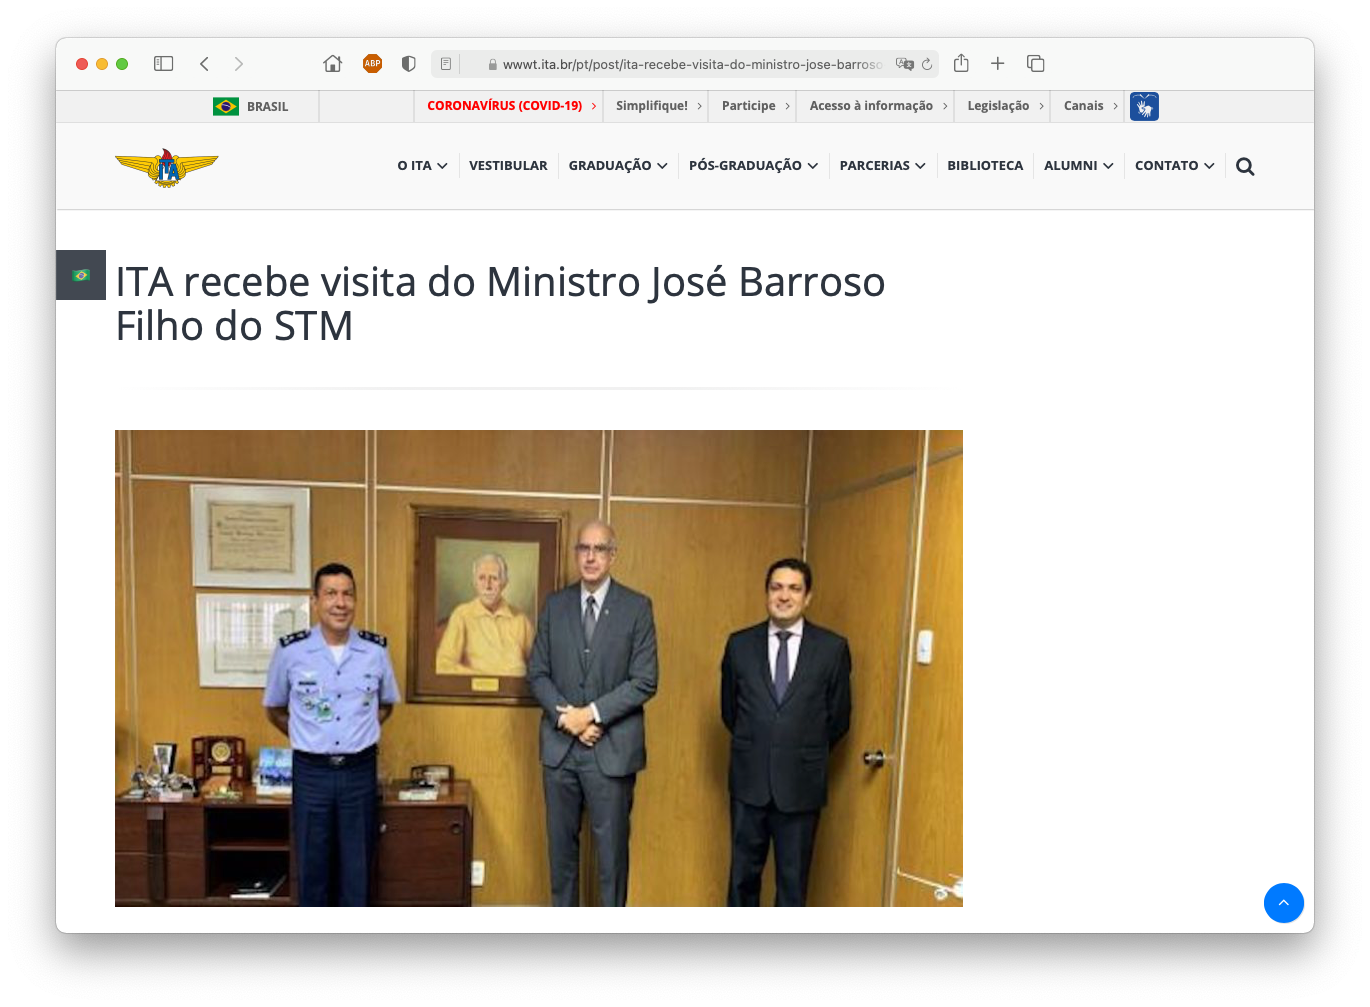
\includegraphics[scale=.25]{post.png}
    \caption{Exemplo de Post}\label{RS0003:fig:post}
\end{figure}

\begin{code}
    \inputminted[label=post.handlebars,firstline=1,lastline=12]{HTML}{../RS0003/anexos/post.handlebars}
    \caption{Post do Portal Institucional - Cabeçalho}\label{RS0003:code:post-head}
\end{code}

No corpo da publicação, logo abaixo dos títulos e do resumo, colocamos um vídeo (se houver, ver linhas $16$ e $17$ da \cref{RS0003:code:post-body}), ou uma imagem (linhas $19$ até $21$ de \cref{RS0003:code:post-body}).

A partir daí, existe a possibilidade de existir um ``\textit{link}'' externo com maiores informações (bloco de código que vai da linha $44$ até $62$) e na linha $64$ é acionado uma ``parcial'' que irá listar arquivos anexos relacionados à esta publicação.

\begin{code}
    \inputminted[label=post.handlebars,firstline=13,lastline=65]{HTML}{../RS0003/anexos/post.handlebars}
    \caption{Post do Portal Institucional - Corpo}\label{RS0003:code:post-body}
\end{code}

Finalmente, a publicação termina posicionando a barra lateral de notícias e destaques (se estiver habilitada, ver linha $71$ da \cref{RS0003:code:post-foot}) e em seguida insere a parcial $subPosts$ que permite que uma publicação tenha diversas outras publicações subordinadas.

\begin{code}
    \inputminted[label=post.handlebars,firstline=66,lastline=92]{HTML}{../RS0003/anexos/post.handlebars}
    \caption{Post do Portal Institucional - Finalização}\label{RS0003:code:post-foot}
\end{code}

No Manual do Editor é demonstrado como criar publicações subordinadas. Um exemplo de publicações subordinadas foi utilizado por exemplo pela Pós-graduação.

Navegue pelo menu até \textit{Pós-graduação / Programas Acadêmicos / Programas / PG/EAM}. Nesta página, o programa PG/EAM apresenta diversas publicações subordinadas: EAM-1, EAM-2, etc., cada uma representando uma área do programa. Cada uma destas áreas tem um único ``\textit{Post}'', e todos eles estão subordinados à uma publicação principal que ao ser apresentada encadeia todas as demais. Na \cref{RS0003:code:sub-post} mostramos a implementação. Este é um exemplo de customização feita para o portal.

\begin{code}
    \inputminted[label=subPosts.handlebars]{HTML}{../RS0003/anexos/subPosts.handlebars}
    \caption{Implementação da Parcial de sub-posts}\label{RS0003:code:sub-post}
\end{code}

\subsubsection{Definição de constantes e a tradução}

Um recurso importante, utilizando principalmente pela tradução dos textos do portal que são fixos, é o uso de constantes.

\begin{forest}
    pic dir tree,
    where level=0{}{
        directory,
    },
    [portal
        [translations
            [en.js, file]
            [pt.js, file]
        ]
    ]
\end{forest}

Uma constante é prefixada pelo termo $translation$, e vem normalmente na forma $translation.<constante>$. Na linha $36$ da \cref{RS0003:code:post-body} temos por exemplo $translation.moreInformation$, ou seja, será apresentada a versão traduzida da linguagem corrente da constante ``$moreInformation$''.

A definição da constante está nos arquivos $translations / en.js$ (\cref{RS0003:code:en}) e $translations / pt.js$ (\cref{RS0003:code:pt}).

\begin{code}
    \inputminted[label=en.js,firstline=1,lastline=10]{JavaScript}{../RS0003/anexos/en.js}
    \caption{Traduções para Inglês}\label{RS0003:code:en}
\end{code}

\begin{code}
    \inputminted[label=pt.js,firstline=1,lastline=10]{JavaScript}{../RS0003/anexos/pt.js}
    \caption{Traduções para o Português}\label{RS0003:code:pt}
\end{code}

Os dois arquivos são praticamente idênticos e o que muda é apenas o conteúdo.

Termos comuns estão logo na raíz. Termos específicos de cada página são agrupados dentro de uma chave específica para a página em questão (ver \cref{RS0003:code:en-iex}).

\begin{code}
    \inputminted[label=pt.js,firstline=11,lastline=25]{JavaScript}{../RS0003/anexos/pt.js}
    \caption{Traduções para o Português}\label{RS0003:code:en-iex}
\end{code}

Na \cref{RS0003:code:en-iex}, a chave para o termo europa é $translation.iex.region.europa$.

Novas páginas podem ser adicionadas (ou até mesmo termos de menus) incluindo novos valores nos dois arquivos. Também é possível acrescentar traduções (o que vai exigir um pouco mais do que apenas acrescentar um arquivo com as traduções).

Já o conteúdo é traduzido por outro mecanismo, o que pode ser visto no manual do Editor, e é processado pelo componente customizado ``\textit{capstone-intl}''.

\subsubsection{Implementação de métodos}

Denominamos métodos requisições especiais que não estão ligadas à uma página diretamente, porém como tudo em \textbf{ExpressJS}, toda requisição termina numa resposta que no caso de um portal na internet é sempre uma página.

\begin{figure}[!ht]
    \centering
    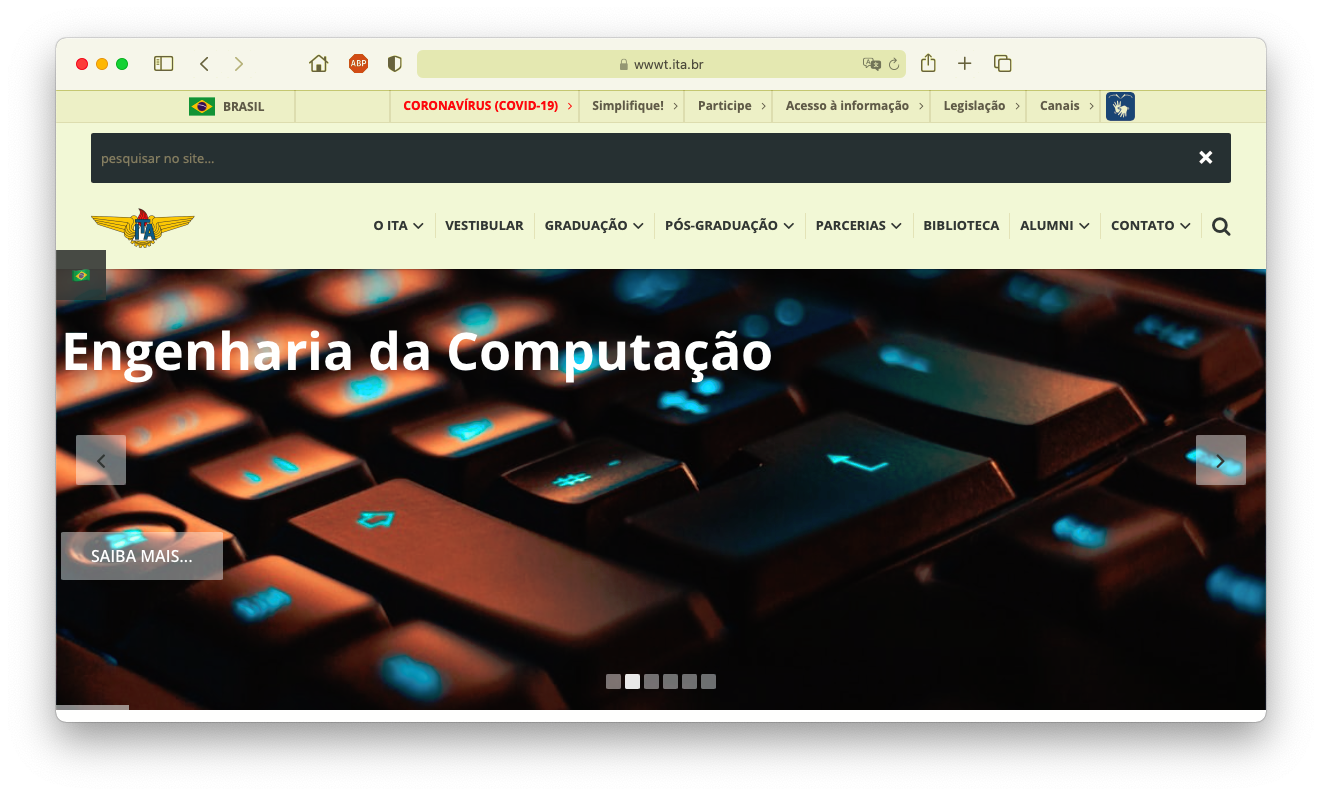
\includegraphics[scale=.25]{search}
    \caption{Entrada do termo de pesquisa}\label{RS0003:fig:search}
\end{figure}

Um caso comum é o botão de pesquisa (a lupa no canto superior direito que podemos ver na \cref{RS0003:fig:search}). Esta opção vai abrir a entrada de valores a serem pesquisados logo acima do menu. Uma vez preenchida, esta entrada irá acionar o método $search$ (linha $106$ da \cref{RS0003:code:def-routes}).

\begin{figure}[!ht]
    \centering
    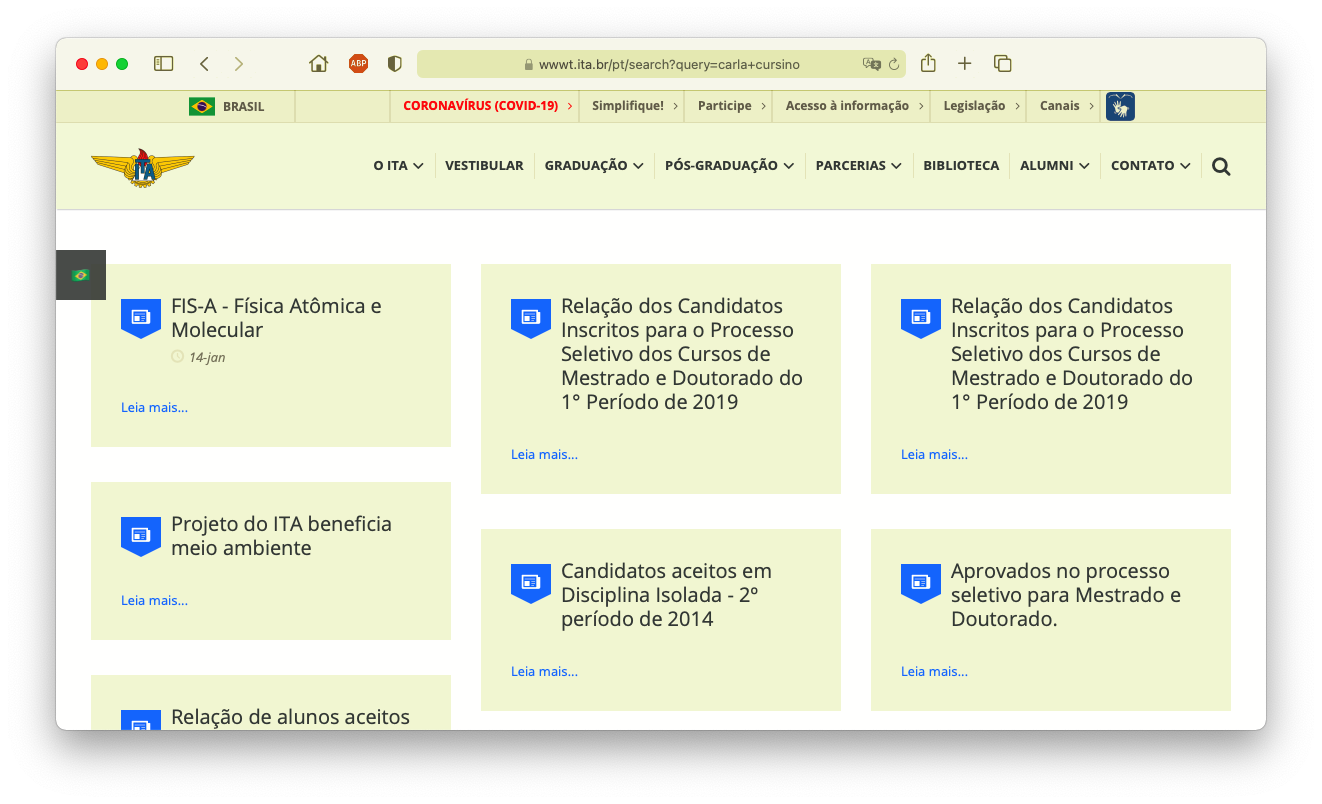
\includegraphics[scale=.25]{result}
    \caption{Resultado de uma pesquisa}\label{RS0003:fig:result}
\end{figure}

O resultado do método é apresentado como uma página (ver \cref{RS0003:fig:result}).

Já o método $download$ que é usado por exemplo pelas publicações que apresentam arquivos para o usuário baixar não resulta em uma página, mas sim num processo que resgata um arquivo que o usuário pode baixar em seu computador. Dependendo do browser e configuração do sistema operacional o arquivo pode ser baixado imediatamente ou pode ser solicitado ao usuário indicar a localização da pasta onde o arquivo será gravado.

\begin{figure}[!ht]
    \centering
    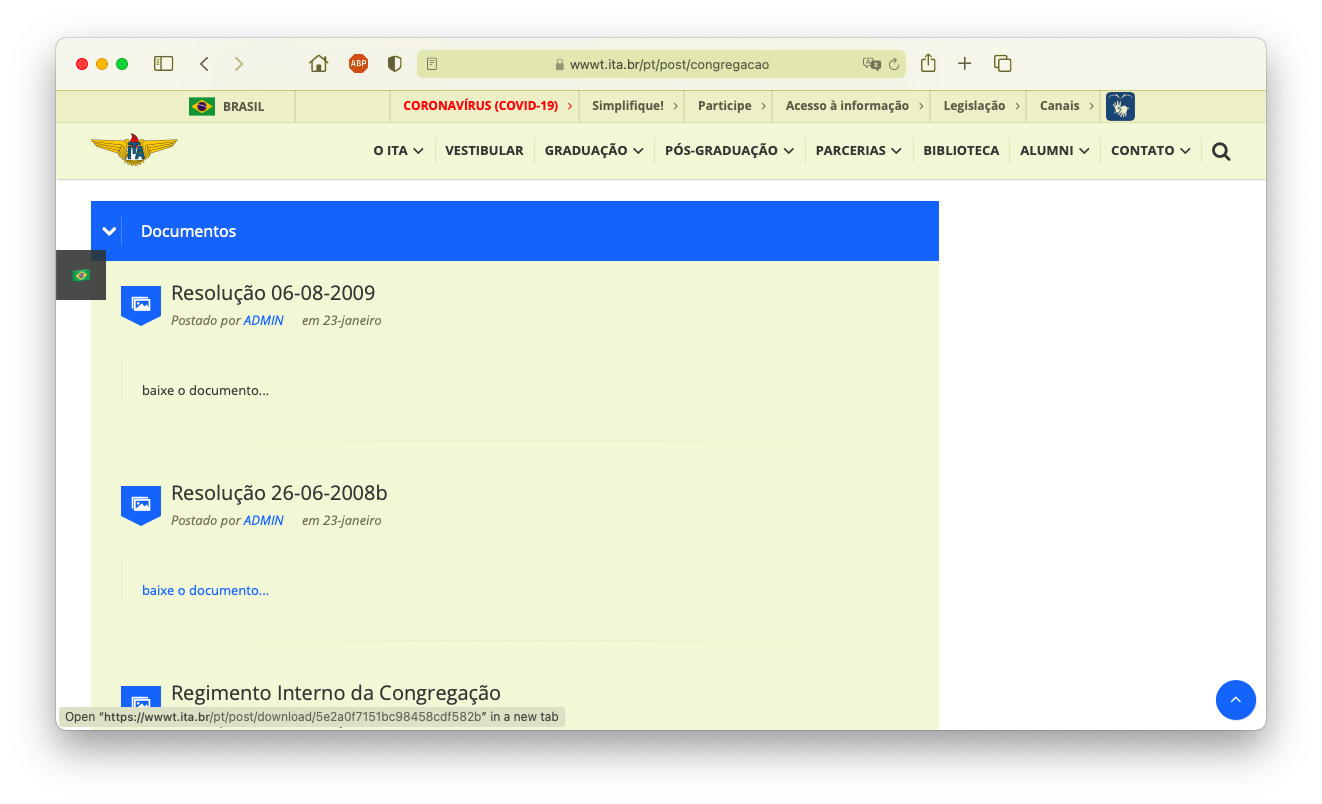
\includegraphics[scale=.25]{download}
    \caption{Exemplo de publicação com arquivos que podem ser baixados}\label{RS0003:fig:download}
\end{figure}

\subsubsection{Definição de modelos de dados}

\begin{forest}
    pic dir tree,
    where level=0{}{
        directory,
    },
    [config
        [atlas.js, file]
        [default.js, file]
    ]
    [models
        [Archive.js, file]
        [Category.js, file]
        [Menu.js, file]
        [Post.js, file]
        [Slider.js, file]
        [Spotlight.js, file]
        [Testimonial.js, file]
        [User.js, file]
    ]
\end{forest}

Modelos de dados são definições de estruturas dos dados que serão armazenados num banco de dados \textbf{MongoDB}. A definição do servidor e banco de dados é feita por meio de arquivos de configuração (ver um exemplo na \cref{RS0003:code:atlas}). Já os modelos são definidos em ``\textit{scripts}'' na pasta $models$.

\begin{code}
    \inputminted[label=atlas.js]{JavaScript}{../RS0003/anexos/atlas.js}
    \caption{Exemplo de definição de servidor e base de dados MongoDB}\label{RS0003:code:atlas}
\end{code}

\begin{code}
    \inputminted[label=default.js,firstline=83,lastline=86]{JavaScript}{../RS0003/anexos/default.js}
    \caption{Definição da pasta de modelos de dados}\label{RS0003:code:def-models}
\end{code}

Na \cref{RS0003:code:def-models} temos na linha $84$ a definição da pasta onde iremos armazenar nossos modelos. E como de praxe, vamos apresentar como exemplo o modelo de uma publicação.

\begin{code}
    \inputminted[label=Post.js]{JavaScript}{../RS0003/anexos/Post.js}
    \caption{Definição do modelo de postagens}\label{RS0003:code:post}
\end{code}

Na \cref{RS0003:code:post} podemos ver as definições que serão usadas pelo modelo da linha $1$ até $13$.

\begin{enumerate}
    \setcounter{enumi}{1}
    \item Acesso ao gerenciador de conteúdo
    \item Acesso às configurações do portal
    \item Tradução de conteúdo
    \item Tratamento de endereços de e-mail
    \item Gerenciamento de arquivos que poderão ser baixados pelo usuário
    \item Tipos de dados
    \item Definição do repositório de dados no \textbf{MongoDB}
    \item Nome do atributo a ser utilizado como identificação das publicações
    \item Aciona a opção do \textbf{Mongoose} de criar atributos que registram data de criação, atualização, usuário que criou e quem atualizou pela última vez
    \item Cria uma chave de acesso a partir do título (que irá se chamar $slug$ - este é um nome padrão para ``\textit{blogs}'')
    \item Ordenação padrão a ser usada quando vários registros forem recuperados pelo \textbf{Mongoose}
\end{enumerate}

Com base no gerenciador de arquivos definido na linha $6$ e do repositório na linha $8$, na linha $15$ inicializamos o gerenciador de arquivos e da linha $17$ até $42$ a estrutura de dados que irão compor uma publicação.

\begin{enumerate}
    \setcounter{enumi}{17}
    \item Título da publicação
    \item Sub-título
    \item Estado da publicação
        \begin{itemize}
            \item ``\textit{Draft}'' - rascunho (padrão) - todo novo registro é criado como ``\textit{draft}''
            \item ``\textit{Published}'' - publicada
            \item ``\textit{Archived}'' - arquivada (não mais publicada)
        \end{itemize}
    \item Autor da publicação (está relacionado com a tabela de usuários do portal)
    \item Data de publicação
    \item Data de aprovação da publicação
    \item Imagem - é um arquivo que deve ser carregado pelo editor
    \item Vídeo - a \gls{URL} que aponta para o vídeo (pode ser no ``YouTube'' ou ``Vimeo'')
    \item Legenda - um texto da imagem e que aparece em algumas apresentações da publicação
    \item Link - uma \gls{URL} para um site externo contendo maiores informações sobre a publicação
    \item Contato - dados de contato para o responsável pela publicação
    \setcounter{enumi}{32}
    \item Conteúdo resumido - um breve resumo que será apresentado no cabeçalho da publicação e em algumas chamadas para o conteúdo
    \item Conteúdo completo - a publicação completa
    \setcounter{enumi}{35}
    \item Categorias - relacionamento com a tabela de Categorias, é um elemento importante para a composição de publicações e controle de acesso aos registros publicados
    \item Downloads - relacionamento com a tabela de Categorias, indica o grupo de arquivos que será listado para que o usuário possa escolher e baixar em seu computador
    \item Panel - painel onde a publicação pode ser apresentada
    \item Continente - usado para o agrupamento de publicações para a ``IPR''
        \begin{itemize}
            \item ``\textit{Americas}''
            \item ``\textit{Europa}''
            \item ``\textit{Asia}''
            \item ``\textit{Africa}''
        \end{itemize}
    \item País - usado para complementar o agrupamento de publicações para a ``IPR''
    \item Pai - esta é a informação utilizada pelo fragmento $subPosts$ que mostramos anteriormente
\end{enumerate}

Da linha $44$ até $46$ definimos um atributo virtual (ver documentação do \textbf{MongoDB}/\textbf{Mongoose} sobre atributos virtuais) que contém todo o texto da publicação (a concatenação de $content.extended$ e $content.brief$).

Em seguida definimos na linha $48$ um relacionamento entre a publicação e o documento que irá conter os ``\textit{Sliders}'' do portal (aquele carrossel de imagens logo no início da página principal).

Na linha $50$ registramos o componente de tradução na estrutura de dados, e por fim, na linha $52$ definimos as colunas que serão apresentadas nas listas do painel administrativo (ver manual do Editor).

Na linha $54$ a estrutura de dados é registrada no \textbf{CapstoneJS} que por sua vez utiliza o \textbf{Mongoose} para ligá-la ao repositório de documentos no \textbf{MongoDB}.

Finalmente, cada atributo possui diversas opções, que devem ser consultadas na documentação do \textbf{Mongoose} e \textbf{MongoDB}.

\subsubsection{Cabeçalhos HTML}

A configuração de cabeçalhos \gls{HTML} é necessária para definir regras e proteções para o usuário do Portal.

Estes cabeçalhos são utilizados pelos navegadores para definir o que é permitido ou não pelo site.

Diversas diretivas são implementadas, seguindo-se recomendações de provedores na Internet e fabricantes de navegadores, e a razão para o uso da maioria foge do escopo deste manual. Aqui iremos apenas esclarecer as escolhas feitas para esta versão do Portal.

\begin{code}
    \inputminted[label=headers.js]{JavaScript}{../RS0003/anexos/headers.js}
    \caption{Cabeçalhos \textbf{HTML}}\label{RS0003:code:headers}
\end{code}

Das linhas $3$ até $22$ temos opções recomendadas para alguns cabeçalhos básicos. Informações detalhadas sobre todos estes cabeçalhos podem ser encontradas no portal \href{https://developer.mozilla.org/en-US/docs/Web/HTTP/Headers}{Mozilla}.

Entre as linhas $23$ e $74$ temos as definições mais importantes. Aqui são definidos os sites que possuem permissão para inserir ``\textit{Scripts}'' nas páginas do Portal e possuem portanto o privilégio de execução na página servida aos usuários. Não só ``\textit{Scripts}'', mas páginas de estilo, fontes e até imagens possuem regras e permissões a serem observadas. Mais uma vez, a documentação do portal \href{https://developer.mozilla.org/en-US/docs/Web/HTTP/Headers}{Mozilla} possui descrição detalhada de como estas informações pode ser modificada com segurança para habilitar ou desabilitar conteúdo de terceiros.